\documentclass[11pt,a4paper]{article}

\usepackage[spanish]{babel}
\usepackage{amsmath,amsfonts, amssymb, amsthm} % Podemos añadir amssymb, amsthm o bm
\usepackage{graphicx, tikz, xparse, array}
\usepackage[top=2cm,bottom=2cm,left=3cm,right=3cm,marginparwidth=1.75cm]{geometry} % Este paquete permite modificar los márgenes del documento
\usepackage[colorlinks=true, allcolors=blue]{hyperref} % Se indica que los hipervínculos van todos en azul
\usepackage{setspace}
\usepackage{caption}
\usepackage{xcolor}
\usepackage{graphicx} % Paquete para incluir imágenes
\usepackage{fancyhdr} % Paquete para cabeceras y pies de página
\usepackage{lipsum}   % Para generar texto de ejemplo
\usepackage[most]{tcolorbox}

\tcbuselibrary{breakable}


%Colores
\definecolor{verdeSuave}{HTML}{6AD58A}
\definecolor{verdeFuerte}{HTML}{206936}
\definecolor{blanco}{HTML}{FFFFFF}
\definecolor{negro}{HTML}{000000}
\definecolor{azulSuave}{HTML}{6ac9d5}
\definecolor{naranjaSuave}{HTML}{d5c06a}
\definecolor{rojoSuave}{HTML}{EF4949}
\definecolor{amarilloSuave}{HTML}{D8E058}


\setstretch{1.2}
\decimalpoint


%\graphicspath{ {images/}}

\title{\textbf{Tema 1: } Teoría de curvas}
\author{Mateo Rama García}


%\date{Fecha}

\begin{document}
  
\begin{titlepage}
  \centering  
  \vspace*{1cm}  % Espacio opcional antes de la imagen
  
\includegraphics[width=0.3\textwidth]{uniovi.jpg} \hspace{2cm}
  
\includegraphics[width=0.3\textwidth]{descarga.jpeg} \\[1cm] 
  \vspace{\fill}% Imagen centrada arriba
  \hrule
  \vspace{0.5cm}
  {\Huge \bfseries Trabajo en grupo\par}
  \vspace{0.5cm}
  {\Large \bfseries Fase I\par}
  \vspace{0.5cm}
  \hrule
  \vspace{1cm}
  {\bfseries PL3-B \\ [3ex]
  Andrés Fernández-Junquera Fernández UO302806\\[3ex]
  Bruno Martín Rivera UO302144\\[3ex]
  Javier Ortín Rodenas UO299855\\[3ex]
  Mateo Rama García UO300710\par} % Nombres centrados
  \vspace{\fill}  % Espacio después de los nombres
  {\Large \textbf{Fundamentos de computadores y redes}\par}
\end{titlepage}



\newpage

\tableofcontents

\newpage


\section{Primera parte}
\subsection{PasswordControl()}
En primer lugar, definimos una constante \texttt{maxChars} con valor 20 para la longitud de los arrays de caracteres que usemos. Estas cadenas solo podrán contener hasta 19 caracteres útiles debido al espacio necesario para \(\backslash \texttt{0}\) que indica el final de la cadena.

Para la primera parte del método, declaramos un array de caracteres \texttt{input1} y almacenamos en él la primera entrada del usuario. Luego, usamos la función \texttt{strcmp} para comparar la entrada con la contraseña. Si el resultado es distinto de 0, es que son diferentes, y prohibimos la entrada.

Para la segunda parte, guardamos la nueva entrada del usuario en el array de caracteres \texttt{input2}. Luego, comprobamos si la longitud del array es menor que 15 o si no coinciden los caracteres en las posiciones 8 y 5. En caso de que no se cumpla alguna de estas condiciones, indicamos que se ha producido un fallo.

\begin{itemize}
  \item Entradas válida: \(\texttt{input2} = \text{''abcdeighijklmnop''}, \hspace{1.5mm} \texttt{input2} = \text{''aaaaabaabaaaaaa''}\)
  \item Entrada no válida: \(\texttt{input2} = \text{''abcd''}, \hspace{1.5mm} \texttt{input2} = \text{''abcdefghijklmnop''}\)
\end{itemize}
\subsection{CountActiveBits()}
Esta función debe pedir dos números enteros sin singo. Posteriormente, debe contar el número de bits activos
que hay en cada número entre la posición 5 y la 8, ambos inclusive. Finalmente, en caso de que el 
número de bits activos entre las posiciones 5 y 8 de los dos números   no sea igual, la función 
imprimirá "No coinciden'' y llamará a la función \texttt{exit()}.
\begin{itemize}
  \item Entrada válida: \texttt{a = 352, b = 448}
  \item Entrada no válida: \texttt{a = 352, b = 0}
\end{itemize}
\subsection{AsmBasedControl()}
\hspace{1mm}
Esta función debe leer tres enteros y pasárselos a \texttt{IsValidAssembly}.
Según la parametrización original del enunciado, esta segunda función debe comprobar que se
cumplan las dos condiciones siguientes:
\begin{itemize}
    \item El bit 8 del segundo número es igual al bit 5 del tercer número
    \item El valor de los 2 bits más bajos del primer número interpretados como 
        binario natural es mayor que 11
\end{itemize}
Como la codificación de 11 en binario natural es \texttt{1011b}, la segunda condición no puede
ocurrir nunca en estas condiciones. Por tanto, escribimos la función para que tome los 4 bits
más bajos del primer entero, los interprete como natural, y lo compare con 11.
\begin{itemize}
  \item  Entrada válida: \texttt{a = -3, b = 403,  c = 56}
  \item Entrada no válida: \texttt{a = 1, b = 7, c = 5}
\end{itemize}

\subsection{ArrayMinMax()}
Este función crea un vector de 3 posiciones de elementos de 8 bits. Después, 
pide por consola los valores para asignar en el mismo, restringiendo los valores de entrada a 
números enteros entre -128 y 127, es decir, los valores enteros codificables con 8 bits con la codificación de complemento a 2. 
Si la entrada no es válida, se informará por consola y se pedirá de nuevo un valor. 
\vspace{1ex}

A continuación, calcula y muestra por consola tanto el valor máximo como el mínimo de los elementos del vector introducidos.
 Si la diferencia entre estos valores no es inferior a $2\cdot \hspace{1mm} $ID[2] (en nuestro caso $2 \cdot 9=18$), se mostrará por pantalla el mensaje ''Fallo'' y se llamará a \texttt{exit()}. 
 \begin{itemize}
  \item Entrada válida: \texttt{arr[0] = -2, arr[1] = 7, arr[2] = 6}
  \item Entrada no válida: \texttt{arr[0] = 2, arr[1] = 5, arr[2] = -20}
\end{itemize}
\newpage
\section{Segunda parte}
Hemos utilizado la versión Visual Studio 2022 para la depuración.
\subsection{Dirección de memoria IsValidAssembly}
Para responder a la pregunta, ponemos un punto de interrupción junto antes de la llamada a la
función \texttt{IsValidAssembly}. A continuación, ejecutamos el programa en modo depuración.
Para poder saber las 
direcciones de memoria, debemos ir a \textbf{Depurar \(\rightarrow\) Ventanas \(\rightarrow\) Desensamblado}. En esta ventana, 
podemos ver las direcciones de memoria a partir de las cuales se sitúa el código de paso de parámetros a la función \texttt{IsValidAssembly}.

\vspace{1ex}
\indent Buscamos la línea de código fuente en la que se realiza la llamada a dicha función. Debajo del la llamada en C++,
nos encontramos con la primera dirección de memoria a partir de la cuál se sitúa el código de paso de parámetros a la 
función en ensamblador al apilar los registros correspondientes (se apilan los parámetros de derecha a izquierda).
En nuestro caso, la dirección de memoria es \(\mathbf{004011E7}\), como se puede observar en la siguiente imagen.
\begin{center}
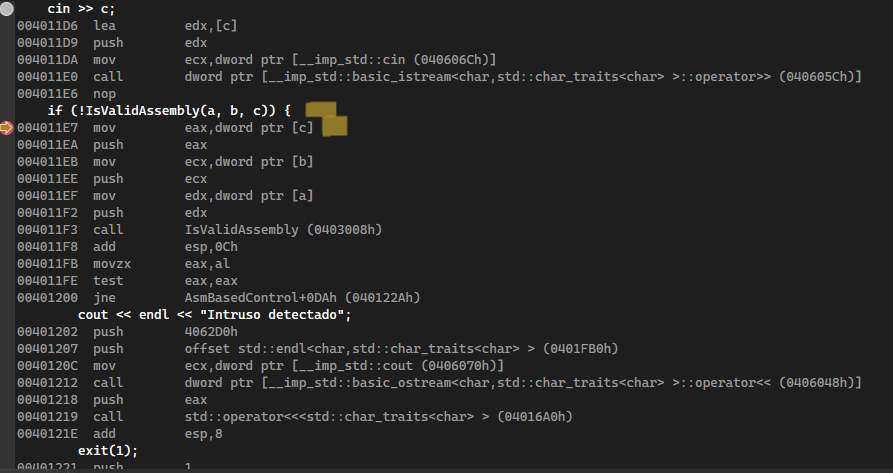
\includegraphics[width=\textwidth]{direccionIsValid.PNG}
\end{center}
\vspace{1ex}

\indent Para poder ver el código máquina y los mnemónicos de la función \texttt{IsValidAssembly}, debemos realizar la ejecución hasta llegar
al punto de interrupción que hemos puesto antes de la llamada a dicha función. Una vez llegamos a este punto, pulsamos la 
tecla \texttt{F11} para ir al código en ensamblador. A continuación, pulsamos click derecho y escogemos la opción \textbf{Mostrar bytes de código}. 
Así, podemos ver tanto los mnemónicos como las instrucciones en código máquina codificado en hexadecimal de la función \texttt{IsValidAssembly}, como se muestra en las siguientes imagenes.
\begin{center}
  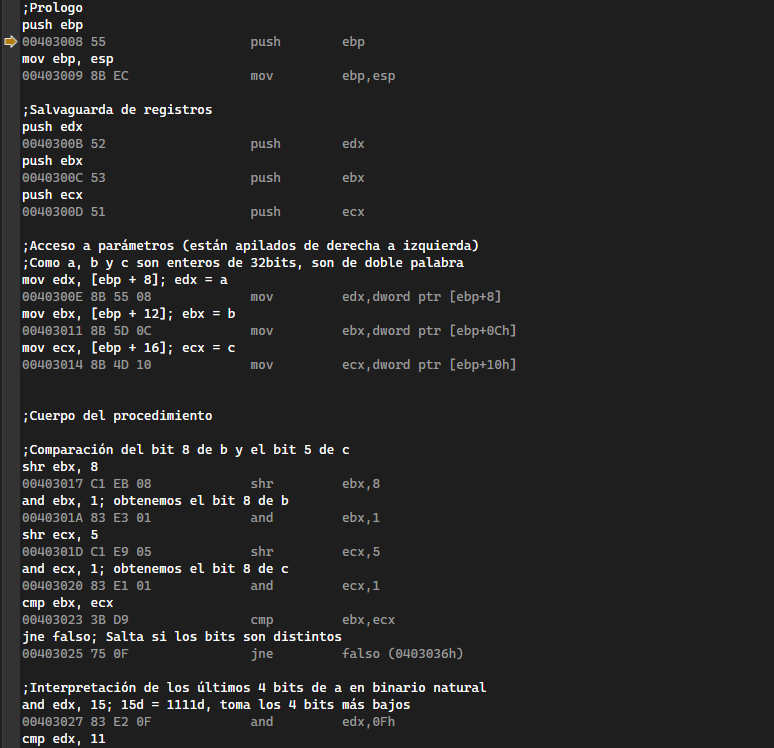
\includegraphics[width=0.8\textwidth]{codigomaquina2.png}
  \end{center}
\begin{center}
  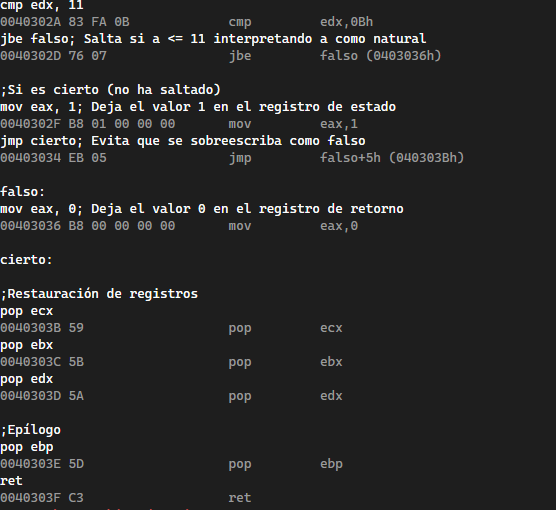
\includegraphics[width= 0.8\textwidth]{codigomaquina1 (1).png}
  \end{center}
\newpage
\subsection{Dirección de memoria PasswordControl}
La pregunta no hace referencia de manera concreta a ninguna de las dos cadenas que se leen en la función
\texttt{PasswordControl}. Por tanto, hemos decidido mostrar ambas direcciones de memoria.

Para saber la dirección de memoria de la primera cadena, debemos poner un punto de ejecución 
después de leerla por terminal. A continuación, ejecutamos el programa en modo depuración y hacemos click 
en la opción \textbf{Ventanas \(\rightarrow\) Depurar \(\rightarrow\) Inspección}. A continuación, añadimos a Inspección 
la variable que contiene la cadena de caracteres y \texttt{\&a} para saber así la dirección de memoria de la cadena.
En nuestro caso, obtenemos el siguiente resultado:
\begin{center}
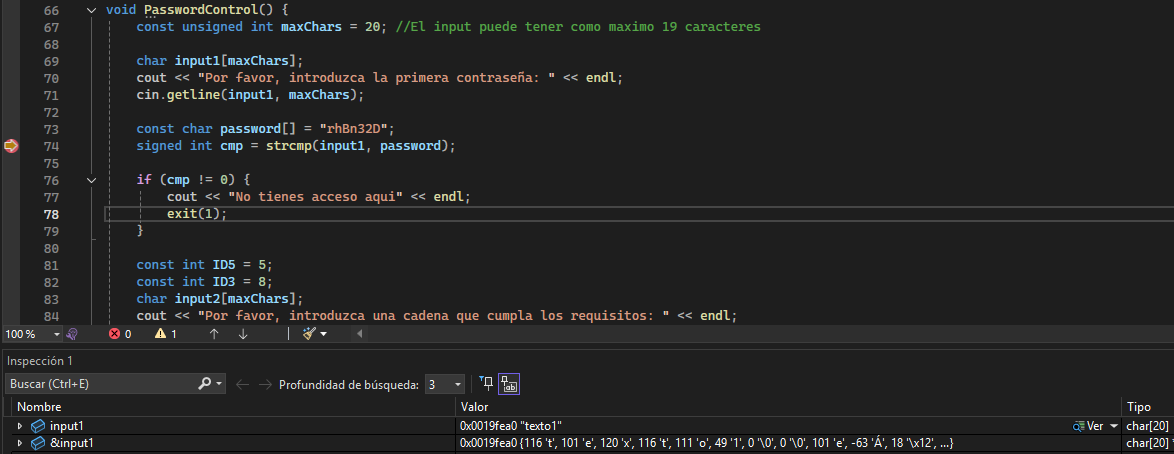
\includegraphics[width=\textwidth]{texto1.png}
\end{center}
Para verlo en memoria, debemos ir a \textbf{Depurar \(\rightarrow\) Ventanas \(\rightarrow\) Memoria}. En esta ventana,
introducimos \texttt{\&a}, para así poder verlo almacenado en memoria, tal y como se muestra en la siguiente imagen.
\begin{center}
  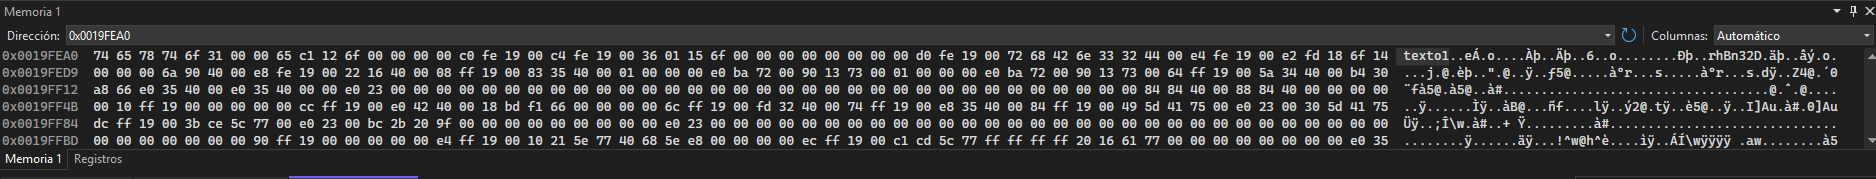
\includegraphics[width=\textwidth]{texto1Memoria.png}
  \end{center}

  \noindent Repetimos el proceso análogamente para la segunda cadena,
  obteniendo lo siguiente:

\begin{center}
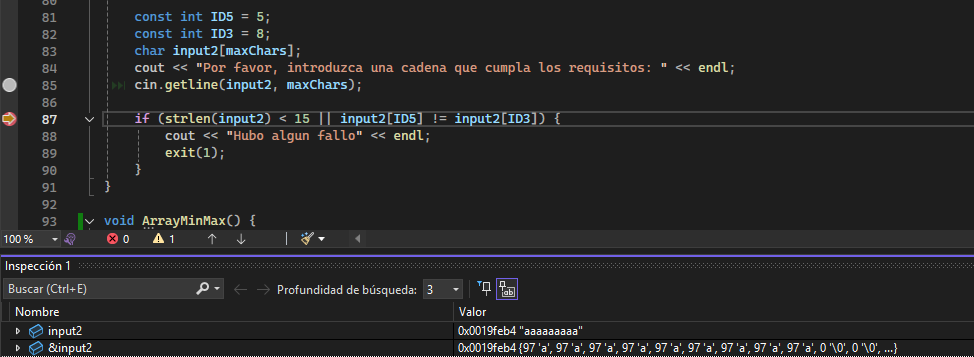
\includegraphics[width=\textwidth]{texto2.png}
\end{center}
\begin{center}
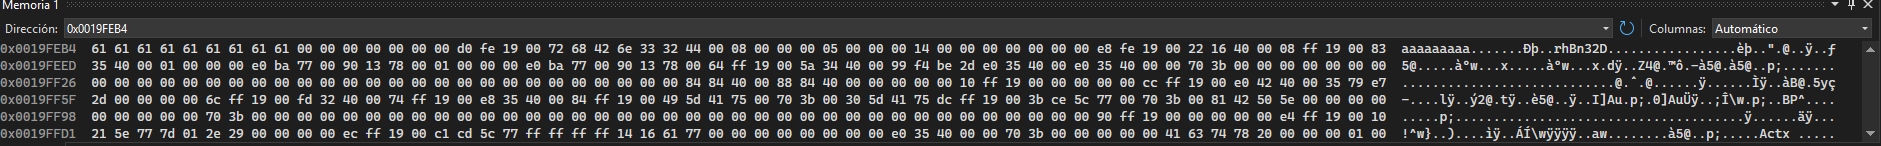
\includegraphics[width=\textwidth]{texto2Memoria.png}
\end{center}

\newpage

\subsection{Marco de pila ArrayMinMax}
Para saber el marco de pila de la función \texttt{ArrayMinMax}, debemos poner un punto de interrupción después de 
leer los elementos del vector. A continuación, ejecutamos el programa en modo depuración y seleccionamos la 
opción \textbf{Ventanas \(\rightarrow\) Depurar \(\rightarrow\) Memoria} y \textbf{Ventanas \(\rightarrow\) Depurar \(\rightarrow\) Registro}. 
En la ventana de memoria, introducimos la dirección de memoria de la variable que contiene el vector; y en la ventana de registro, vemos en qué dirección 
de memoria se encuentra el puntero de pila.
\begin{center}
  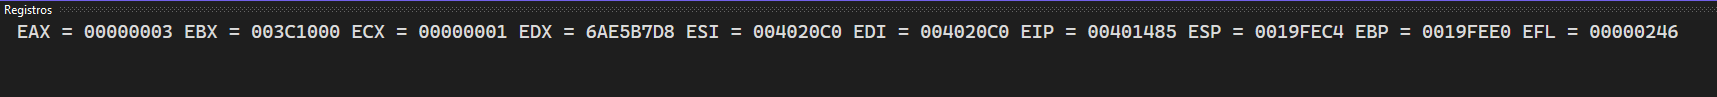
\includegraphics[width=\textwidth]{VentanaRegistros.png}
  \end{center}

\indent En nuestro caso, tenemos que la dirección de memoria de la variable que contiene el vector es \(\mathbf{0x0019FED8}\), la dirección de memoria del puntero de pila es \(\mathbf{0x0019FEE0}\), y la dirección de retorno es \(\mathbf{0x0019FEE4}\).
Los resultados fueron interpretados a partir de la siguietne imagen:
\begin{center}
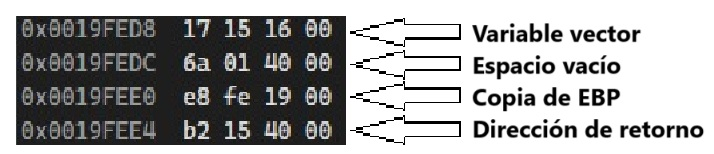
\includegraphics[width=\textwidth]{VentanaMemoria.jpg}
\end{center}

Nótese que hay un espacio vacío para futuras variables locales que se van a usar más adelante en la ejecución del método.


\subsection{Acceso de lectura ArrayMinMax}
Para explicar el acceso de lectura a un elemento del vector, debemos poner un punto de interrupción en la lectura 
de sus elementos. En nuestro caso, cuando se lee el elemento cero del vector para inicializar al máximo.
 A continuación, ejecutamos el programa en modo depuración y, haciendo click derecho sobre el código, vamos al desensamblado. Como se 
 Imagen del desensamblado obtenido:
 \vspace{1ex}
 \begin{center}
  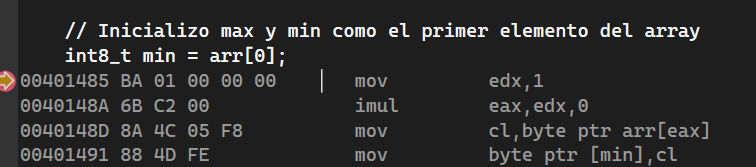
\includegraphics[width=\textwidth]{VentanaDesensamblado.png}
 \end{center}
 \vspace{1ex}
 Explicación de la imagen:
 \begin{enumerate}
  \item En la primera línea, asigna el valor 1 al registro \texttt{edx}.
  \item En la segunda línea, multiplica el valor del registro \texttt{edx} (en nuestro caso el 1) por el valor 0 (ya que estamos accediendo al primer elemento del vector) y asigna el 
  resultado al registro \texttt{eax}.
  \vspace{3ex}

  \item Mueve la información almacenada en la posición \texttt{eax} del vector (en nuestro caso es la posición 0) a los 8 bits más bajos del registro \texttt{c}. Se omite la letra \texttt{ecx} de \texttt{e} para acceder a la 
  palabra más baja del registro, y ponemos \texttt{l} en lugar de \texttt{x} para acceder a los 8 bits más bajos, de ahí que se escriba \texttt{cl} en lugar de \texttt{ecx}.
  \item Mueve la información almacenada en la parte baja del registro \texttt{ecx} a la variable local de un byte denominada \texttt{min}.
 \end{enumerate}

\newpage

\section{División del trabajo}
A la hora de organizar el trabajo en equipo, nos reunimos todos para aportar ideas y
pensar en común los cuatro métodos. Después de plantear varias ideas y ponernos de acuerdo 
en cómo hacer cada método, nos dividimos la creación de código de la siguiente manera, siempre 
siguiendo el guion que habíamos acordado en un principio:
\begin{itemize}
  \item Andrés Fernández-Junquera Fernández: \texttt{ArrayMinMax()}
  \item Bruno Martín Rivera: \texttt{PasswordControl()}
  \item Javier Ortín Rodenas: \texttt{AsmBasedControl()}
  \item Mateo Rama García: \texttt{CountActiveBits()}
\end{itemize}

\indent Cada alumno programó su respectiva función de manera independiente y realizó una serie de pruebas para comprobar
el correcto funcionamiento del código. 
\vspace{2ex}

A continuación, trabajamos en conjunto para responder a las cuestiones, explicar el código, y redactar la memoria. También, 
se han contabilizado las horas de trabajo de cada uno de los integrantes del grupo, siendo estas las siguientes:
\begin{itemize}
  \item Andrés Fernández-Junquera Fernández: 4 horas
  \item Bruno Martín Rivera: 4 horas
  \item Javier Ortín Rodenas: 5 horas y media
  \item Mateo Rama García: 5 horas y media
\end{itemize}

\end{document}
